%%%%%%%%%%%%%%%%%%%%%%%%%%%%%%%%%%%%%%
%		Basic configuration
%%%%%%%%%%%%%%%%%%%%%%%%%%%%%%%%%%%%%%
\documentclass[10pt, oneside, fleqn]{report}
\usepackage[no-math]{fontspec}

\usepackage{polyglossia}
\setdefaultlanguage{french}
\setotherlanguages{english}



%%%%%%%%%%%%%%%%%%%%%%%%%%%%%%%%%%%%%%
%		Various packages
%%%%%%%%%%%%%%%%%%%%%%%%%%%%%%%%%%%%%%
\usepackage{microtype}
\usepackage{graphicx}
\usepackage[german=swiss]{csquotes}
\usepackage{calc}
\usepackage[usenames,dvipsnames,svgnames,table]{xcolor}
\usepackage{setspace}

\usepackage{shapepar}


%%%%%%%%%%%%%%%%%%%%%%%%%%%%%%%%%%%%%%
%		Colors
%%%%%%%%%%%%%%%%%%%%%%%%%%%%%%%%%%%%%%
%\definecolor{mainColor}{RGB}{150, 150, 150} % a sort of light gray
\definecolor{mainColor}{RGB}{211, 47, 47} % some dark red
\definecolor{secondColor}{RGB}{255, 167, 38}



%%%%%%%%%%%%%%%%%%%%%%%%%%%%%%%%%%%%%%
%		Font
%%%%%%%%%%%%%%%%%%%%%%%%%%%%%%%%%%%%%%
\defaultfontfeatures{Ligatures=TeX}
\frenchspacing
% Normal font
\setsansfont{Lato Light}[
	Numbers=OldStyle,
	BoldFont=Lato Regular,
	ItalicFont=Lato Light Italic,
	BoldItalicFont=Lato Italic
]
% Normal font
\setmainfont{Lato Light}[
	Numbers=OldStyle,
	BoldFont=Lato Regular,
	ItalicFont=Lato Light Italic,
	BoldItalicFont=Lato Italic
]
% Font for chapter number
\newfontfamily{\upperNumber}{Lato Light}[
	BoldFont=Lato Regular,
	ItalicFont=Lato Light Italic,
	BoldItalicFont=Lato Italic
]



%%%%%%%%%%%%%%%%%%%%%%%%%%%%%%%%%%%%%%
%		Layout
%%%%%%%%%%%%%%%%%%%%%%%%%%%%%%%%%%%%%%
\usepackage[
	xetex,
	papersize={216mm, 303mm},
	ignoreheadfoot,
	left=3.8cm,
	right=3cm,
	top=3.3cm,
	bottom=3.8cm,
	nohead,
	marginparwidth=0cm,
	marginparsep=0mm
]{geometry}
\setlength{\skip\footins}{1cm}
\setlength{\footnotesep}{2mm}
\setlength{\parskip}{1ex}
\setlength{\parindent}{0ex}




%%%%%%%%%%%%%%%%%%%%%%%%%%%%%%%%%%%%%%
%		Links
%%%%%%%%%%%%%%%%%%%%%%%%%%%%%%%%%%%%%%
\usepackage{hyperref}
\hypersetup{
	colorlinks=true,
	linkcolor=blue,
	linktoc=all,
	urlcolor=blue,
	citecolor=blue,
	filecolor=blue
}



%%%%%%%%%%%%%%%%%%%%%%%%%%%%%%%%%%%%%%
%		TikZ
%%%%%%%%%%%%%%%%%%%%%%%%%%%%%%%%%%%%%%
\usepackage{tikz}
\usetikzlibrary{shapes}



%%%%%%%%%%%%%%%%%%%%%%%%%%%%%%%%%%%%%%
%		Bibliography
%%%%%%%%%%%%%%%%%%%%%%%%%%%%%%%%%%%%%%
\usepackage[
	sorting=none,
	defernumbers=true,
	isbn=false,
	backend=biber
]{biblatex}
\addbibresource{./bibliographie/biblioTypoNature.bib}



%%%%%%%%%%%%%%%%%%%%%%%%%%%%%%%%%%%%%%
%		Itemize and consort
%%%%%%%%%%%%%%%%%%%%%%%%%%%%%%%%%%%%%%
\def\labelitemi{---}
\usepackage{enumitem}
\setlist[itemize]{nosep}
\setlist[description]{nosep}
\setlist[enumerate]{nosep}


\newcommand{\inColor}[1]{{\bfseries\color{LimeGreen}#1}}

\pagestyle{empty}


\begin{document}
	
	\newgeometry{bottom=2cm, right=2.7cm}
	
	
	\begin{tikzpicture}[remember picture, overlay]
		\node[xscale=-1] at (current page.center) {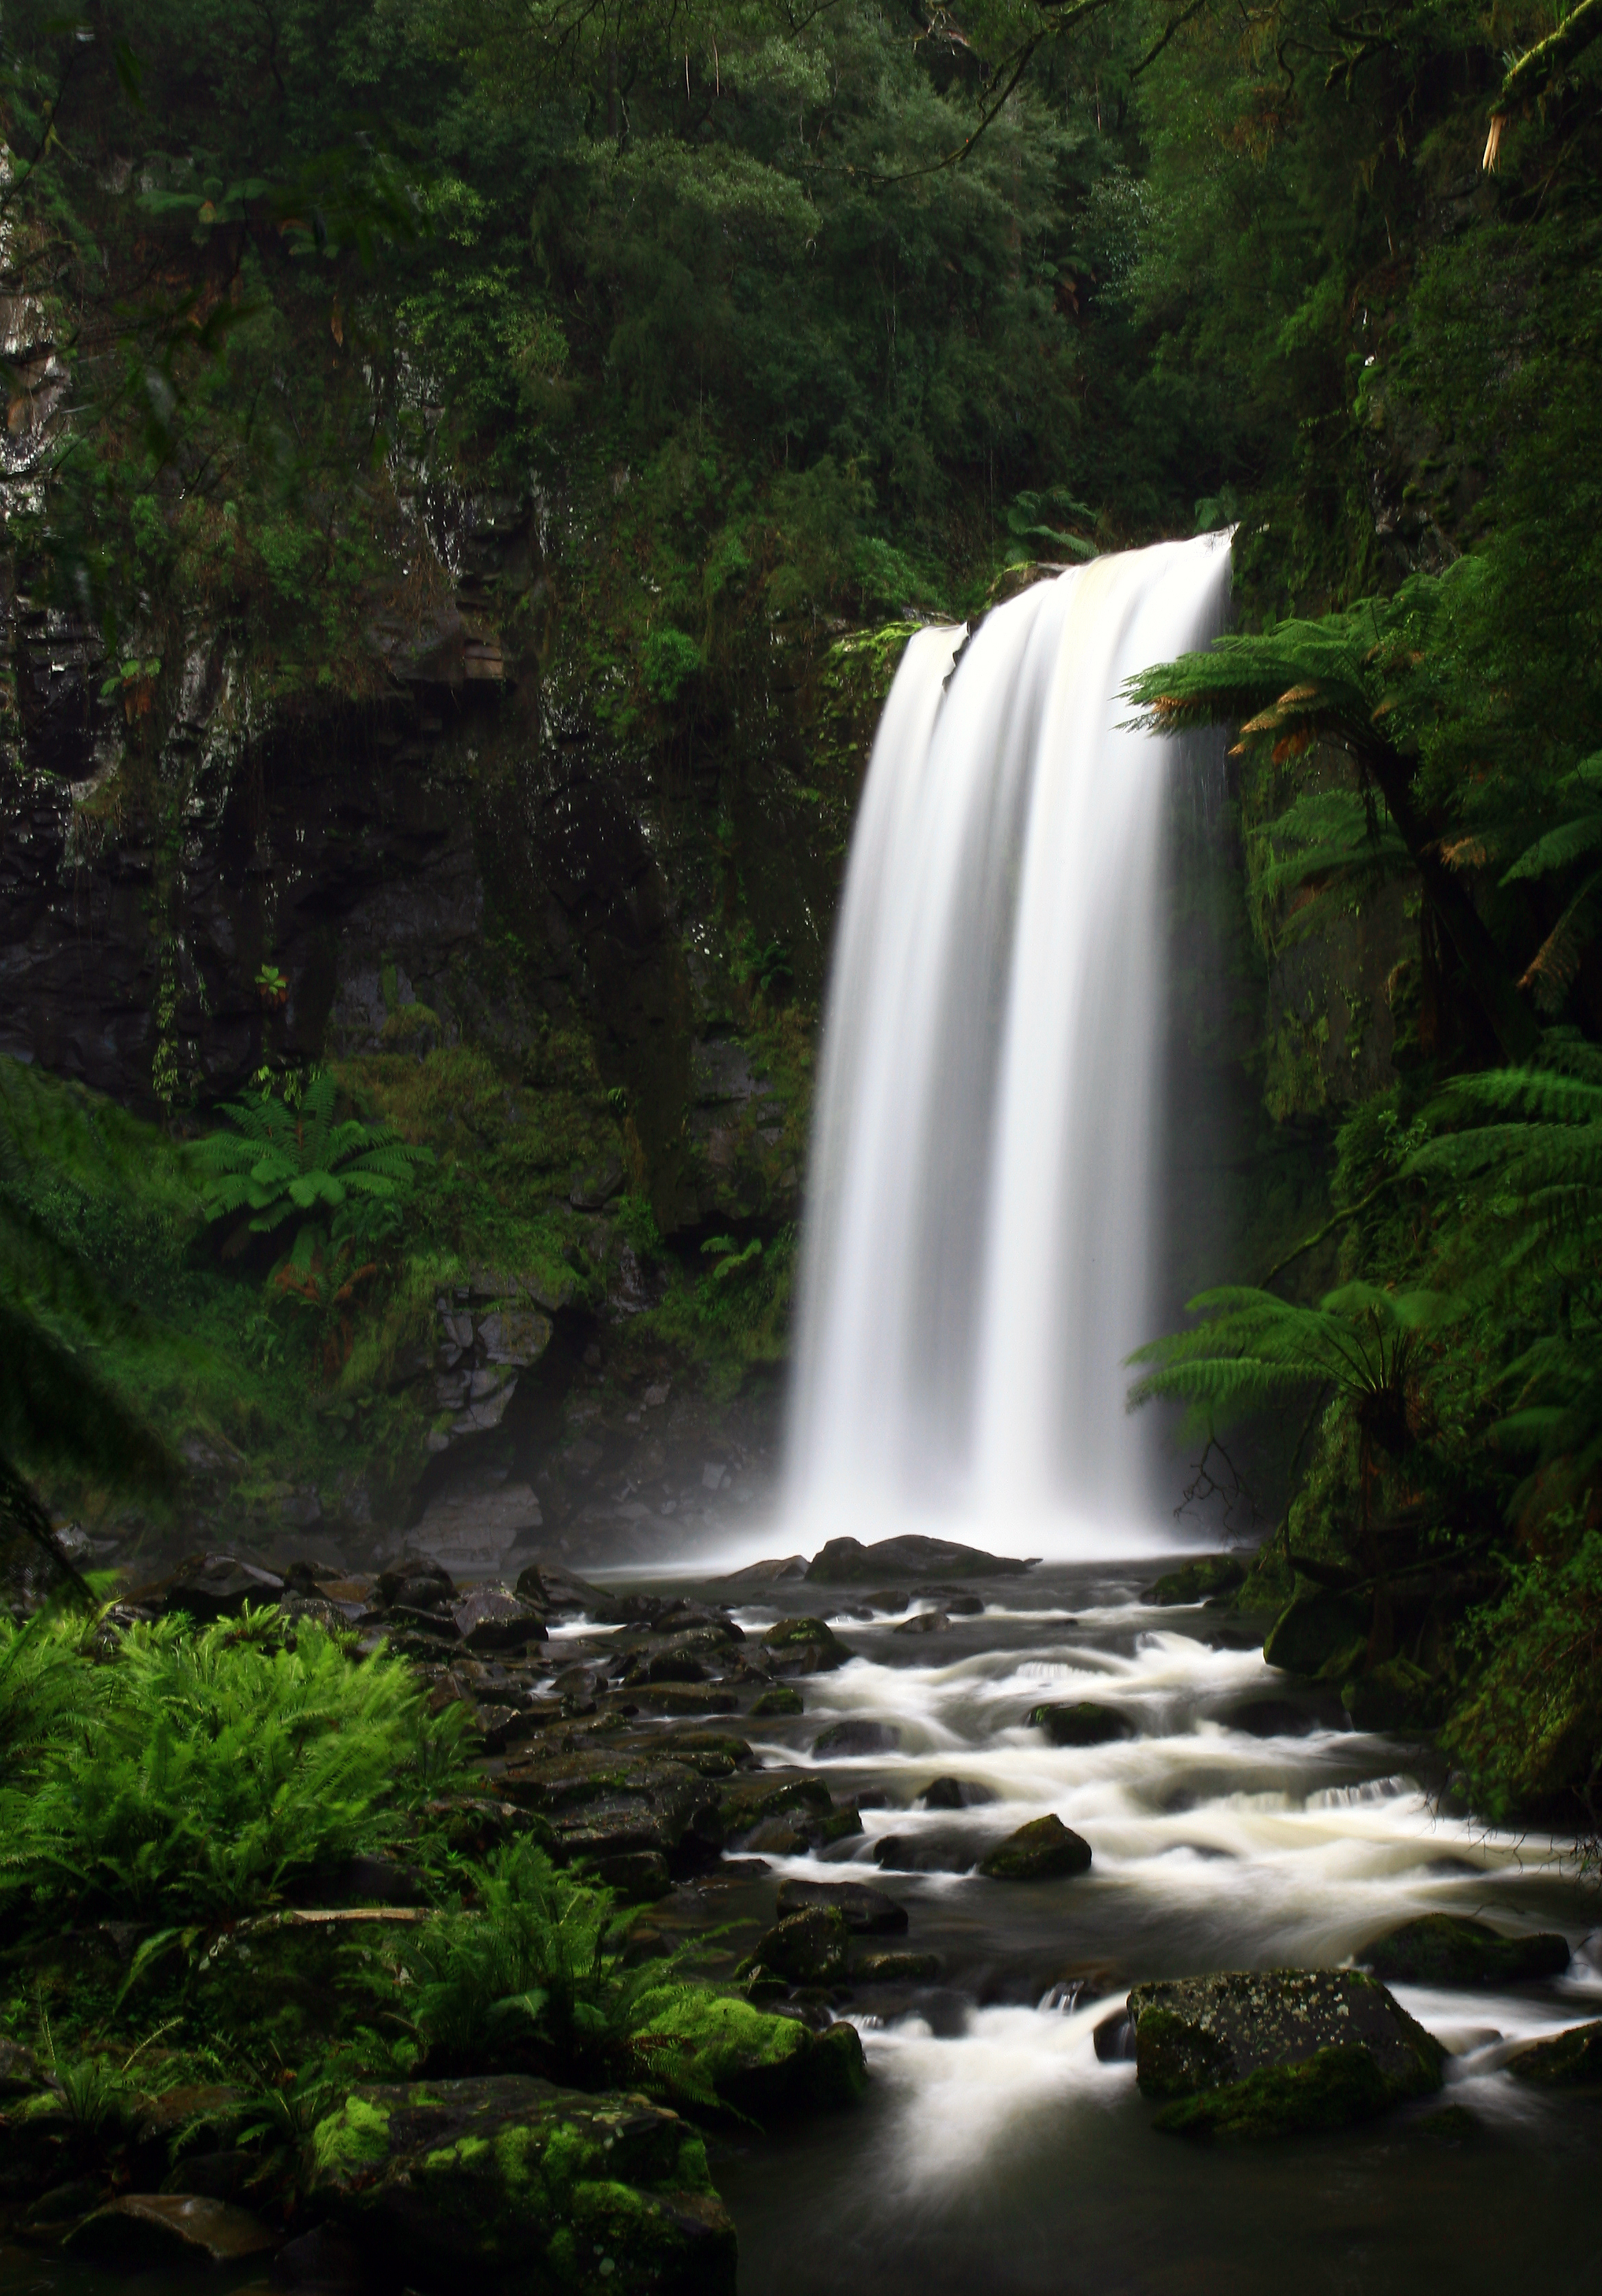
\includegraphics[width=\paperwidth]{images/hopetounFallsDark2.jpg}};
	\end{tikzpicture}
	
	\hfill\parbox{.5\textwidth}{
		\begin{flushright}
			\begin{spacing}{2}
			\fontsize{1cm}{2em}\selectfont
			\color{White}\fontspec[BoldFont=Lato]{Lato Light}
			\enquote{Quand l'homme\\n'aura plus de\\place pour\\la Nature,\\peut-être\\la {\bfseries\color{LimeGreen}Nature}\\n'aura-t-elle\\plus de place\\pour l'homme}\\[1.5ex]
			--- Stefan Edberg
			\end{spacing}
		\end{flushright}
	}
	
	\vfill
	\begin{center}
		\begin{tikzpicture}
			\node[circle, minimum size=2cm, fill=LimeGreen, inner sep=0mm] (node name) {
				\begin{minipage}{4.6cm}
					\vspace*{1mm}
					\shapepar[4.6cm]{\circleshape} \footnotesize \textbf{Nature}, \textbackslash na.tyʁ\textbackslash, subst. fem. (du latin \textit{natura}): Au sens large, elle désigne les êtres et les choses qui constituent l'univers. On utilise parfois ce terme pour parler du monde naturel, physique et matériel, considéré en dehors de l'être humain. Elle peut aussi se référer aux phénomènes et lois du monde physique qui maintiennent l'ordre des choses et des êtres. L'étude de la Nature constitue la plus grande partie des sciences.
				\end{minipage}
			};
		\end{tikzpicture}
	\end{center}
	
	\newpage
	\restoregeometry
	
	\textbf{Photo:} \fullcite{FullForce_B}
	
	\textbf{Définition:} \fullcite{Nature_} et \fullcite{Nature_a}
	
\end{document}